% This is samplepaper.tex, a sample chapter demonstrating the
% LLNCS macro package for Springer Computer Science proceedings;
% Version 2.20 of 2017/10/04
%
\documentclass[runningheads]{llncs}
%
\usepackage{graphicx}
\usepackage{amsmath,amssymb,amsfonts}
\usepackage{algorithm}
\usepackage{algorithmic}
% 支持多行注释的宏包
\usepackage{verbatim} 
\usepackage{CJKutf8} % 兼容中文

% 支持插入并排图片的4个宏包
\usepackage{float} 
\usepackage{subfigure}
\usepackage{caption}
% Used for displaying a sample figure. If possible, figure files should
% be included in EPS format.
%
% If you use the hyperref package, please uncomment the following line
% to display URLs in blue roman font according to Springer's eBook style:
% \renewcommand\UrlFont{\color{blue}\rmfamily}

\begin{document}
%
\title{Senti-weibo: Sentiment Analysis Platform for Weibo}
%
%\titlerunning{Abbreviated paper title}
% If the paper title is too long for the running head, you can set
% an abbreviated paper title here
% double-blind
\author{xxx\inst{1}}
%
% \authorrunning{F. Author et al.}
% First names are abbreviated in the running head.
% If there are more than two authors, 'et al.' is used.
%
\institute{
xxx
\email{lncs@springer.com}\\
\url{http://www.springer.com/gp/computer-science/lncs}
}
%
\maketitle              % typeset the header of the contribution
%
\begin{abstract}
Microblogging sentiment analysis aims at exploring people's opinion on social networks such as Twitter and Weibo. Existing work mainly focus on the English corpus based on distant supervision, which ignores the noise data in corpus and internationalization. In this work, we propose an iterative method to purify noise and expand corpus based on distant supervision. Although there is a lot of work on Chinese Weibo sentiment analysis, it's hard to find available large scale corpus for application and evaluation. Therefore, we formulate the problem of corpus construction into an information retrieval problem and construct a Weibo sentiment analysis corpus called Senti-weibo2019 based on the iterative method above. We also release a weibo pre-processing toolkit in order to unify the pre-processing rules of Weibo text. Eventually, we apply these works to implement the real-time Weibo sentiment analysis platform: Senti-weibo, which serves to analyze and track the sentiment of Weibo topics.

\keywords{Corpus construction \and Sentiment analysis platform \and Distant supervision \and Weibo pre-processing.}

\end{abstract}

\section{Introduction}
% 介绍微博情感分析的意义
Weibo, the most popular microblogging social network in China, has 465 million Monthly Active Users in March 2019. People can express their opinion about breaking news, current affairs, politics and other topics. Massive traffic even led to multiple downtimes on Weibo server. These subjective data are rich in sentiment information, which brings great convenience to the research of sentiment analysis.

% 介绍情感分析与语料库的中外现状与不足之处
Sentiment Analysis (or Opinion Mining) aims at using information technologies understand the opinion of others. Sentiment analysis on Twitter has made significant progress in sentiment corpus. Most of the methods for constructing sentiment corpus\cite{iosifidis2017large} use the Distant Supervised Learning method\cite{go2009twitter}, which labels the sentiment of Twitter with emotion words such as ``:-) '' and ``:( ''. However, emotion words cannot fully represent the sentiment polarity in tweet, and corpus mentioned above are actually corpus with noise. In the field of the Chinese Weibo sentiment analysis, Chinese Opinion Analysis Evaluation (COAE2014) \cite{Yang2015Task} provide a collection of 40,000 weibos (equals tweet of Twitter) for research. Compared with Twitter sentiment analysis, the field of Weibo sentiment analysis lacks a large-scale and complete corpus.

% 介绍文本预处理
Pre-processing for Twitter data usually used for denosing and dimensionality reduction. The experiment results of \cite{haddi2013role} show that appropriate text pre-processing methods can significantly enhance the classifier's performance. \cite{bao2014role} discusses the role of pre-processing in Twitter sentiment analysis and show the results that precision rises when some methods are applied. A
Chinese Weibo text pre-processing is more complex than English text for the reason that Chinese do not use spaces to mark potential word-boundaries. We are also short of a unified rule for Weibo text cleaning. For example, supposing that we have applied a couple of word segmentation tool and cleaning rule to preprocess Weibo dataset and train a corresponding classifier. Then if we want to make full use of this classifier in online environment, the segmentation tool and cleaning rules should be consistent with training environment. Otherwise, a large number of unknown words will be generated.

% 介绍 system
Sentiment analysis plays an import role in many systems. In review-related system, sentiment analysis can be used to analyze the polarity of reviews. \cite{song2019distilling} focuses on document-level sentiment classification to evaluate the overall sentiment score of products. A characteristics of microblogging sentiment analysis is the data visualization. Compass \cite{paul2017compass} provides an interactive web visualization system to visualize the event of US Presidential Election 2016 in spatio-temporal domain. To the best of our knowledge, no open-sourced sentiment analysis application provides real-time analysis for the weibo topic.

In this work, we aim at the design of real-time sentiment analysis system, and center on the construction of large-scale and complete Chinese Weibo sentiment analysis corpus. Our works are summarized below:

\begin{itemize}
\item We formulate the problem of corpus construction into an information retrieval problem and propose an Iterative Distant Supervised Learning(IDSL) method to construct Weibo Sentiment Analysis Corpus: Senti-weibo2019\footnote{Available at: http://bit.ly/2IEzTw1}, a collection of 671,053 weibos without duplication.
\item We unify weibo pre-processing rules and package it into a toolkit in Python: weibo-preprocess-toolkit\footnote{https://pypi.org/project/weibo-preprocess-toolkit}, which is applied for weibo cleaning and segmentation. Experiment shows that the consistent text pre-processing rules in the training and online environment can maximize the performance of model.
\item As shown in Fig.~\ref{fig:system-screenshot}, we design a real-time Weibo Sentiment Analysis Platform called Senti-weibo\footnote{http://sentiweibo.top} to analyze and track the sentiment of weibo topics. A Weibo Topic Spider is designed to crawl real-time weibos for analysis. In particular, we take the topic of ``China-US Trade'' and ``Huawei'' as concrete examples and track the sentiment trend of them.
\end{itemize}


\begin{figure}[htp]
\begin{center}
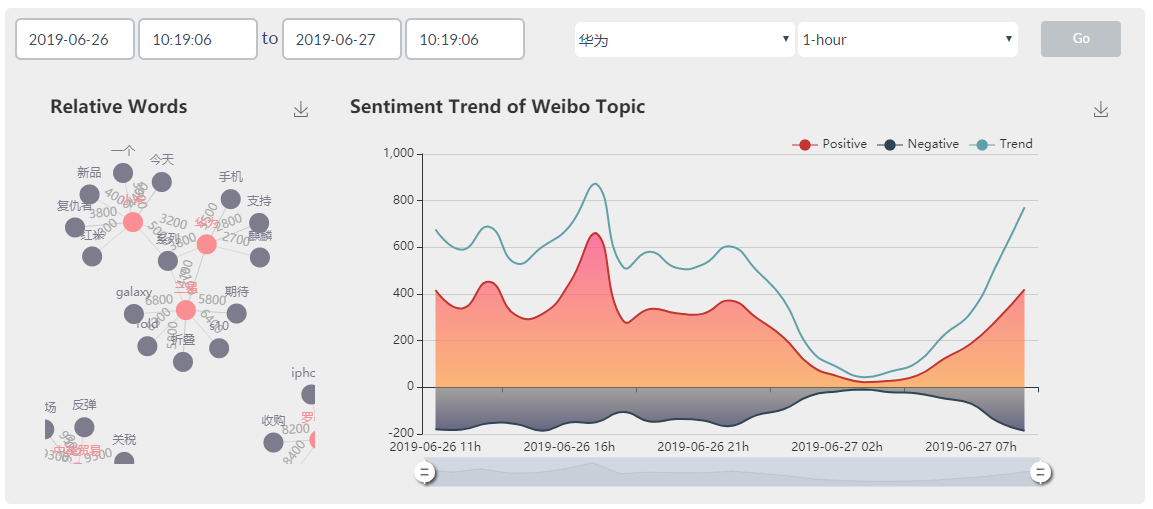
\includegraphics[width=0.7\textwidth]{images/system-screenshot.png}
\caption{Screenshot of Senti-weibo}
\label{fig:system-screenshot}
\end{center}
\end{figure}

\section{Data Collection and Pre-processing}

\subsection{Data Collection}

% 介绍微博爬虫
In this work, we aim at the sentiment analysis of Weibo topics and construction of sentiment corpus. So we need two types data from Weibo: topic data and sentiment data. Weibo topic data serves to real-time sentiment analysis. We choose to design Weibo Spider personally for the reason that it is hard to get the API authority from Weibo. As for the sentiment data, the previous retrieval methods mostly sample the sentiment weibo from existing weibo dataset according to typical emojis. However, we cannot update and iterate the sentiment dataset unless new weibo datasets are continuously open-sourced. Relying on Weibo Topic Spider, we crawl specified topic of Weibo and accumulate data for the iteration of corpus.

\subsection{Weibo Pre-processing}

% 介绍微博预处理工具
A unified weibo pre-processing rule can keep the training environment and online environment consistent, so as to maximize the performance of the model. We take the Chinese segmentation tools by way of example. Six segmentation tools are used to cut the test dataset, then we apply the pre-trained model segmented by jieba to classify the test set and get the precision on each test set. As shown in the Fig.~\ref{fig:segmentation-tools-precision}, test set segmented by jieba get the highest precision, which corresponds to the segmentation tool of training dataset. In fact, jieba is not the best Chinese segmentation tool, but the consistent rules in the training and test environment maximize the performance of model.

\begin{figure}[htp]
\begin{center}
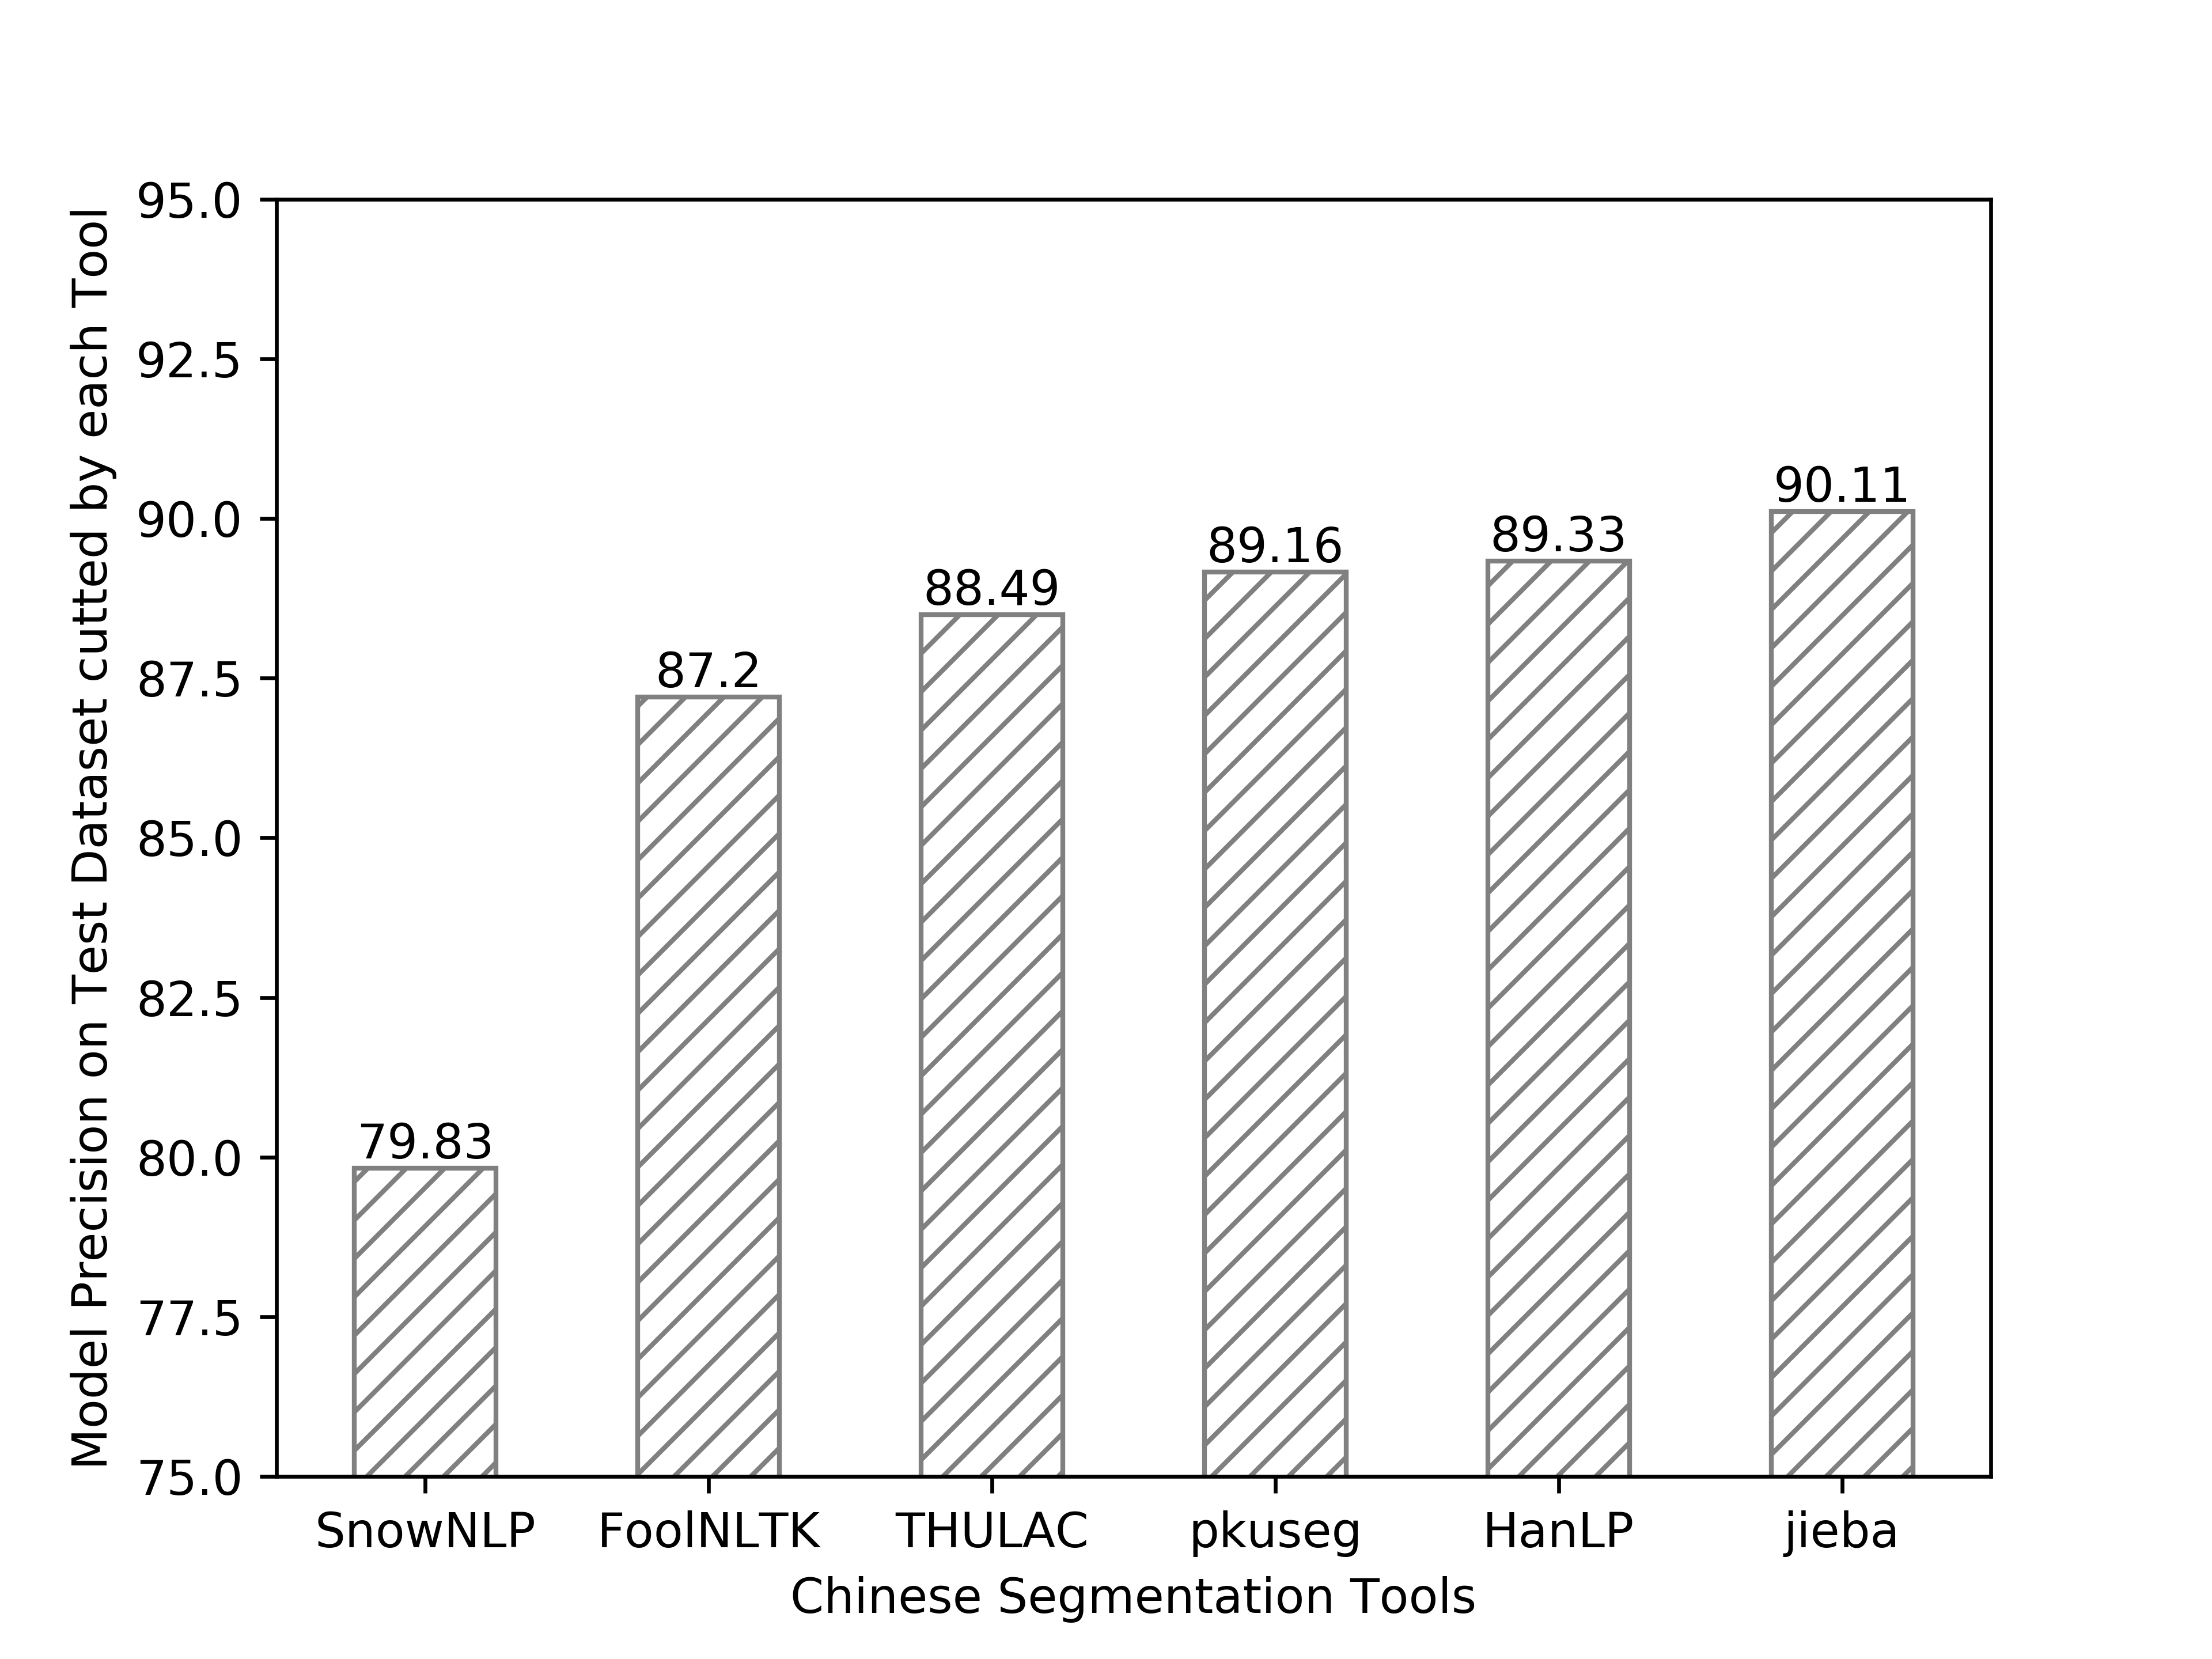
\includegraphics[width=0.38\textwidth]{images/model-precision-on-test-dataset-cutted-by-each-tool.png}
\caption{Model precision on test dataset cutted by each tool}
\label{fig:segmentation-tools-precision}
\end{center}
\end{figure}

In the pre-processing of Weibo text, we summarize the noise rules and sort out Weibo stop words in the form of regular expression. The NTU Sentiment Dictionary(NTUSD) \cite{ku2006opinion} is added into jieba to improve the precision of segmentation. We also convert the text from Traditional Chinese to Simplified Chinese in advance, and consider the cleaning of special characters to further reduce the noise of Weibo text. Finally, we package the pre-processing rules mentioned above and release the weibo-processing-toolkit in Pypi. 

\section{Corpus Construction and Model Training}

The problem of corpus construction can be explained to a query problem in Information Retrieval. The two basic measures we want to optimize are precision and recall. In this work, we first query sentiment weibos from public dataset with emojis and sentiment dictionary. Secondly, We keep querying sentiment weibos using Weibo Topic Spider with sentiment words to continuously iterate the corpus.

\newtheorem{myDef}{Definition}

\begin{myDef}
Formally, given a database $D$(public dataset or Weibo server),the retrieved weibos as $R(D)$.  $Precision$ is the sentiment relevant weibos of $R(D)$, $Recall$ is the sentiment weibos in $R(D)$ retrieved from $D$:

\scriptsize{ % 公式字体大小
% 空格:\ 
% 公式对齐:align* 就是用来包裹需要对齐的公式, 以 & 开头,以 \\ 结尾,最后一行不需要 \\
\begin{align}
&Precision = \frac{\#\left ( sentiment\ weibos\ retrieved \right )}{\#\left ( retrieved\ weibos \right )} = P\left ( sentiment | R(D) \right ) \\
&Recall = \frac{\#\left ( sentiment\ weibos\ retrieved \right )}{\#\left ( sentiment\ weibos \right )} = P\left (retrieved\ sentiment | D\right )
\end{align}
} % end of 字体大小
\end{myDef}

In order to construct a corpus and train a model with high performance, we need to optimize the $Precision$ for high precision of sentiment classification model and improve the $Recall$ for high robustness of model.

\subsection{Corpus Initialization and Iteration}

We follow the similar procedure as in \cite{go2009twitter} to initialize the corpus. Weibo sentiment corpus construction based on emotion words can be reduced to a query problem, using emotion words as search query from Weibo server or existing dataset. We develop rigorous rules to recall sentiment weibos from existing Weibo dataset. First, we manually select 40 typical positive emojis and 27 typical negative emojis with intense sentiment to recall sentiment weibos from existing weibo dataset. In particularly, weibos with two opposite emojis are filtered out. Second, the NTUSD serves to further filter the dataset. If a weibo contains sentiment words in NTUSD that are emotional different from the emojis in weibo, it will also be filtered out. Rigorous query rules ensure the sentiment precision of recalled weibos and we initialize the Weibo sentiment corpus with 663,535 weibos. The sentiment classifier trained on this corpus has the initial precision of 87.04 on test dataset. The test dataset comes from COAE2014 and we manually labeled 1,790 weibos. The training algorithm of classifier is fastText\cite{joulin2016bag}, which is a lightweight and efficient library for text representation learning and text classification.

\subsection{Corpus Iteration and Model Training}
% 补充:采用 Distant Supervision Learning 构建的语料库都是包含有噪声的语料库。
Corpus built with Distant Supervised Learning method\cite{go2009twitter,iosifidis2017large} are corpus containing noise. We propose an Iterative Distant Supervised Learning(IDSL) method to purify and expand the corpus dynamically. Fig.~\ref{fig:model-iteration} presents an overview of IDSL. This iterative method consists of the following four modules:


\begin{equation} 
IDSL = (C, L, Q, P)
\end{equation}

\begin{itemize}

\item \textbf{C, Classifier} Sentiment classifier is the training result of corpus. 

\item \textbf{L, Labeled Corpus} Actually, it should be the labeled corpus with noise.

\item \textbf{Q, Query Func} Query Function is the Weibo Topic Spider with specific combinations of sentiment words as topic.

\item \textbf{P, Purify Func} Purify Function serves to filter the noise samples in corpus.

\end{itemize}


% 筛子筛面粉的比喻,将后面的 4 个 subsubsection 融入这一段
In fact, the iteration can be interpreted as a process of sifting sands out of flour. Given a sieve and some flour to be sifted, our goal is to sift out the sand with sieve. The difficulty is that the holes on the sieve are not all small holes, there will always be sands mixed into flour. We propose three ways to optimize these problems. 

First, we can try to sift more times to filter out more sands. Second, we continuously improve the sieve during the iteration. Purify Function plays an important role in this part. Classifier trained by initialized corpus will lead to over-fitting iff we apply it to purify the corpus. So we divide the corpus into training set and verification set, and sample subset of training dataset to train the classifier many times. Multiple classifiers are used to verify the sentiment label of the verification dataset, and then sift out the samples whose classification results are not unified. The last method is to optimize the quality of the flour to be sieved in advance, that is, to improve the quality of the data from the data source. Query Function can help to continuously recall new high-quality data to guarantee the robustness of the model. We use spider with two related sentiment words as topic to recall sentiment weibos from Weibo server. We select the banned words released by Xinhua News Agency as negative seed words and manually select some typical positive words as positive seed words. Then, we use word2vec to generate the similar sentiment words about each seed word. Combining two sentiment words generated by one seed as a query can improve the sentiment precision of recalled weibos than using one word as query, and the similarity of two words can make sure the recall rate, which can prevent situation where no weibo is recalled from Weibo server. 

\begin{figure}[htp]
\begin{center}
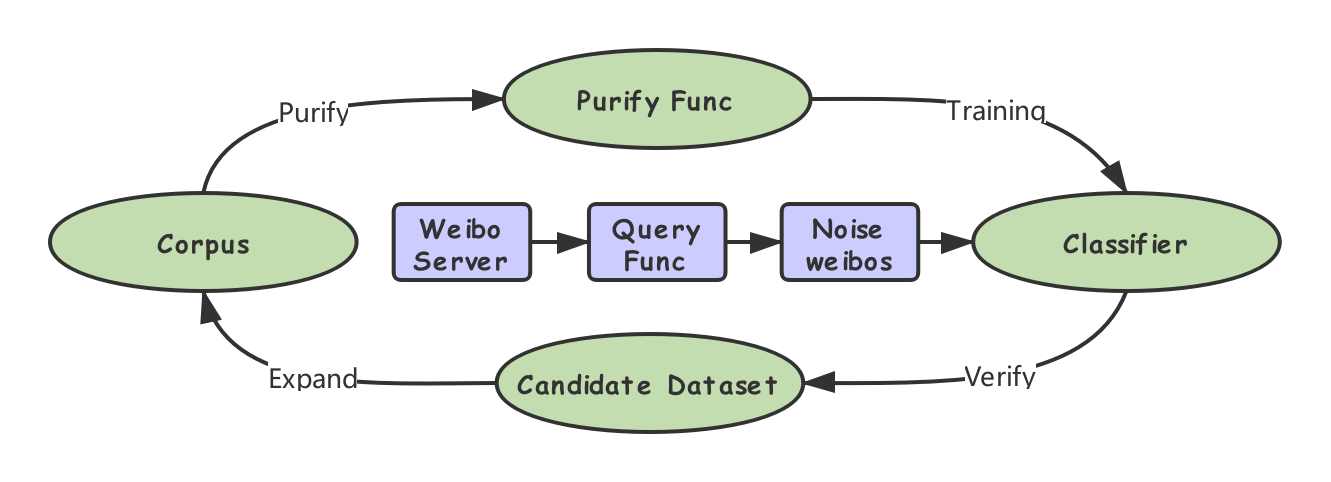
\includegraphics[width=0.40\textwidth]{images/Model-Iteration-2.png}
\caption{Iteration of Corpus}
\label{fig:model-iteration}
\end{center}
\end{figure}

After several rounds of iteration, the precision of model has increased by 3.07 points. Finally, we build a Weibo Sentiment Analysis Corpus: Senti-weibo2019, a collection of 671,053 weibos. The sentiment classification model trained on this corpus reaches the precision of 90.11. 

\section{Weibo Sentiment Analysis Platform}


We design a demonstration platform called Senti-weibo to present our works mentioned in each section. Senti-weibo is a real-time Weibo sentiment analysis platform, Fig.~\ref{fig:Senti-weibo} presents an overview of this platform's architecture.

\begin{figure}[htp]
\begin{center}
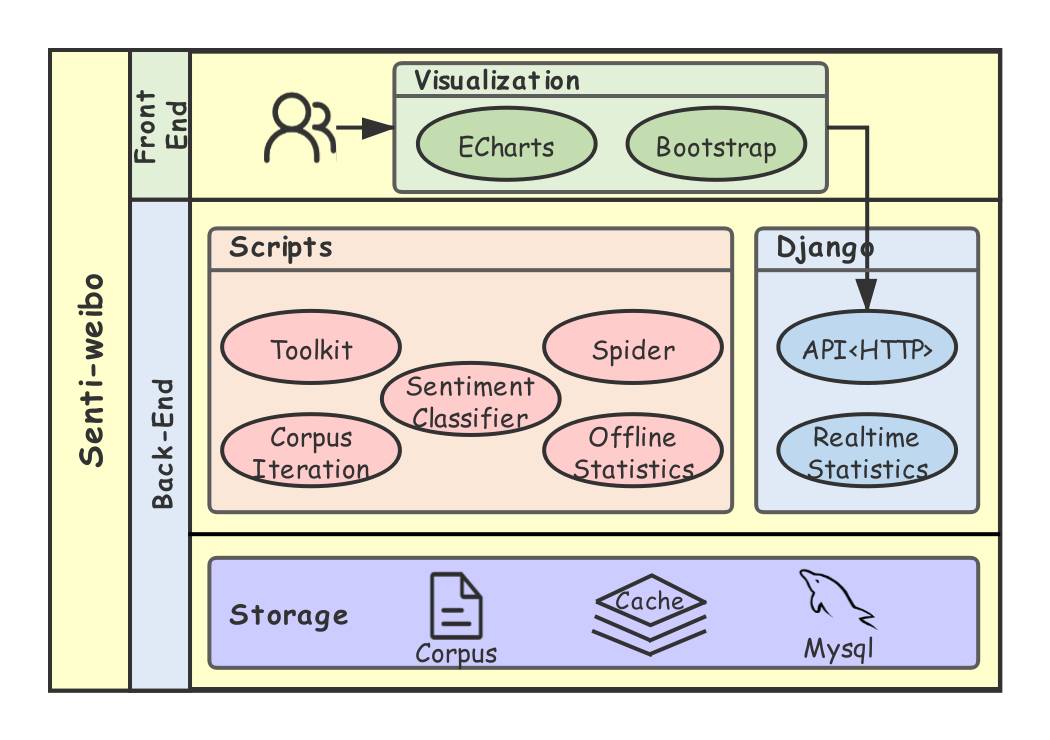
\includegraphics[width=0.44\textwidth]{images/Architecture-of-Senti-weibo-3.png}
\caption{Architecture of Senti-weibo}
\label{fig:Senti-weibo}
\end{center}
\end{figure}

\begin{comment}
常用选项[htbp]是浮动格式:
『h』当前位置。将图形放置在正文文本中给出该图形环境的地方。如果本页所剩的页面不够,这一参数将不起作用。
『t』顶部。将图形放置在页面的顶部。
『b』底部。将图形放置在页面的底部。
『p』浮动页。将图形放置在一只允许有浮动对象的页面上。
\end{comment}

\begin{figure*}[ht]
\centering  %图片全局居中
\subfigure[Senti-weibo's topic trend]{
\label{fig:Senti-weibo's topic trend}
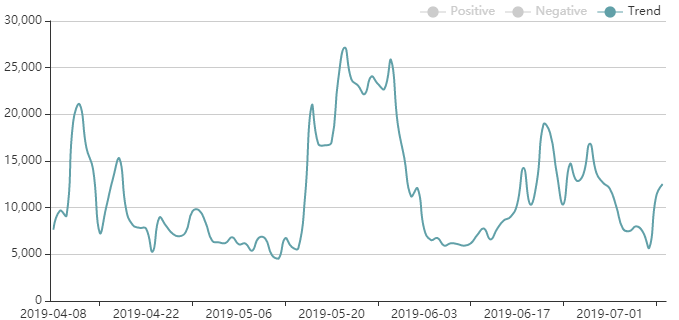
\includegraphics[width=5.7cm, height=3.0cm]{images/huawei-echarts-trend.png}}
\subfigure[Weibo-Index's topic trend]{
\label{fig:Weibo-Index's topic trend}
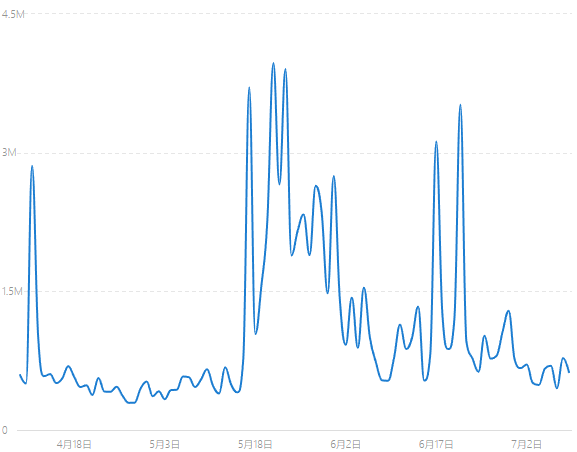
\includegraphics[width=5.7cm, height=3.0cm]{images/weibo-index-trend.png}}
\caption{Comparison of two platforms}
\label{fig:topic-trend-of-huawei}
\end{figure*}

\begin{figure*}[ht]
\centering  %图片全局居中
\subfigure[Huawei]{
\label{fig:huawei-1day}
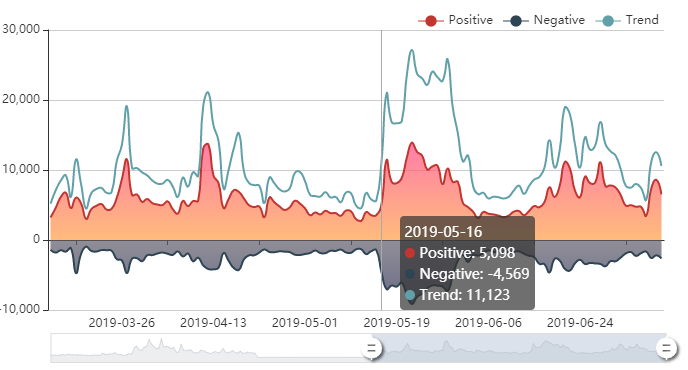
\includegraphics[width=5.7cm, height=3.0cm]{images/huawei-alert.png}}
\subfigure[China-US trade]{
\label{fig:trade-5min}
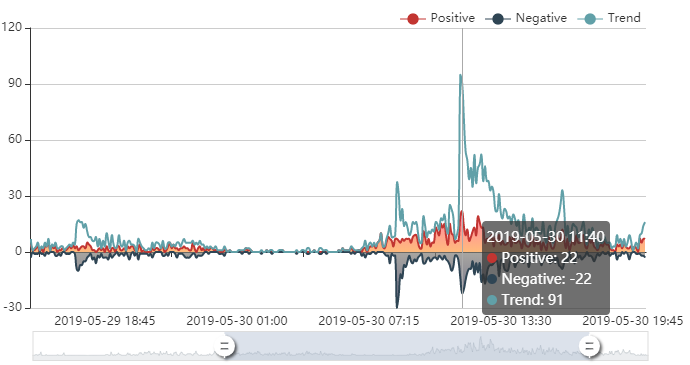
\includegraphics[width=5.7cm, height=3.0cm]{images/china-us-detate-5min.png}}
\caption{Temporal sentiment analysis}
\label{fig:sentiment-trend}
\end{figure*}

\subsection{Overview of Senti-weibo}

% 结构图重新画,介绍重新写,加一些技术名词
The back end of platform starts with the collection of topic data with Weibo Topic Spider. Spider continuously crawls the weibos to ensure the platform's real-time track of topic. After the pre-processing, newly collected weibos are stored in cache for the sentiment classification. Scripts module provides several scripts to support platform. For example, the Offline Statistics script is used to perform offline statistics on the results of sentiment classification such as hourly or daily statistics, and save the statistical results into database, which accelerates the request from front end. 

In the front end of platform, interactive UI provides interface to interact with web server in back end. We provide multiple query options, including topics, time ranges and query frequencies. User can combine these options and send the request to obtain real-time or history sentiment analysis of topics. After the response from back end, ECharts \cite{li2018echarts} is applied to render statistics data to visualize the sentiment. In particular, the platform's minimum frequency for temporal sentiment analysis is 5 minutes, which means that we can track the sentiment trends of any topics 5 minutes ago.

\subsection{Temporal Sentiment Analysis}

We select two representative topics in the past half year: ``Huawei'' and ``China-US Trade'', to demonstrate the sentiment analysis of Senti-weibo. We compare the official results of topic trend provided by Weibo-Index with statistics generated by Senti-weibo. As shown in Fig.~\ref{fig:topic-trend-of-huawei}, we visualize the topic trend of Huawei from April to July, and Senti-weibo's result matches to the Weibo-Index to a large extent. 

Fig.~\ref{fig:sentiment-trend} shows the results of platform's temporal sentiment analysis of two specified topics. Fig.~\ref{fig:huawei-1day} represents the daily sentiment trend of Huawei from March to July. We can see that the negative sentiment of Huawei has increased since May 16, which accurately reflects the event that Huawei is added to the Entity List. Fig.~\ref{fig:trade-5min} shows the sentiment trend of China-US trade from May 29 to May 30 in a five-minutes frequency, which corresponds to the intense emotional changes of Chinese netizens to the anchors' debate between China and US. After this debate, China-US's relation tend to ease and the sentiment of netizens became normal, which can be reflected by visiting the Senti-weibo. We also open-source weibo data for two topics collected from April to July.

\section{Conclusion}

In this work, we construct the real-time sentiment analysis platform: Senti-weibo, and introduce some modules in platform, including the Weibo sentiment analysis corpus and weibo pre-processing toolkit. The details of Senti-weibo can be available on GitHub\footnote{https://github.com/wansho/senti-weibo}, including regexes of Weibo stop words, sentiment seed words, test dataset and others. Next, we will continue to optimize the corpus using IDSL method and account for different sentiment levels \cite{le2017ontology}.


%
% ---- Bibliography ----
%
% BibTeX users should specify bibliography style 'splncs04'.
% References will then be sorted and formatted in the correct style.
%
\bibliographystyle{splncs04}
\bibliography{dasfaa2020}

\end{document}
